\section{Evaluation}\label{sec:eval}
\subsection{Setup}
\textbf{Simulator.} ns-3.46 with lr-wpan: CSMA/CA, acknowledgements and retransmissions, the channel and radio of
Section~\ref{sec:model}. The network is deployed and organised by one binary, the pass by a second, and the ground
transport by a third; all three are frozen for the campaign.

\textbf{Maps and regimes.} Three maps on a non-convex domain with lakes, with 8, 12 and 15 clusters (capacitated
$k$-medoids, at most 80 cells each) and 45, 66 and 92 critical cells; the smallest has 617 cells and 13\,086 nodes. Four
A2G regimes, $R_{50}=1016$, 498, 199 and 99\,m. Cluster geometry, CHs and critical cells are the same for all schemes.

\textbf{Schemes.} \emph{\lmtour{}+River} and \emph{\chord{}+River} (Section~\ref{sec:flight}), with River's repair
enabled and per-critical-cell windows. \emph{DTSP-N+River}: a Dubins path that enters the disc $B(k,\xi)$ of
\emph{every} critical cell, crossing each cluster once, followed by River; it isolates the value of River from that of
the path. \emph{FC+DTSP-N}: no ground cooperation; the query is coded with an ideal rateless code ($\epsilon=0.05$); Team~1
flies a DTSPN through groups of nearby critical cells (group radius 200, 300 or 400\,m, whichever gives the shortest
plan) and orbits each group until every member has heard enough, in expectation, with a margin of three standard
deviations per image; its receptions follow the channel model rather than a packet-level ns-3 pass. \emph{No broadcast}:
Team~2 alone visits every critical cell with the full reference (a rotary-wing TSP), as an upper reference.

\textbf{Replications.} Ten simulation seeds; a seed fixes the fading of the pass, the shadowing and fading on the ground
and the MAC draws. Each seed is one ns-3 run per cluster and 100 paired draws of the matching layer, shared by all
schemes. The campaign was stopped at 81\,\% of its jobs, so a setting has 6--10 seeds. Confidence intervals are Student-$t$
intervals over per-seed means, because the 100 draws of a seed share one network realisation.

\subsection{Mission time}
Table~\ref{tab:tstar} and Fig.~\ref{fig:tstar} report $T^\star$. \lmtour{}+River is the fastest scheme in every setting.
Against FC+DTSP-N it is 10--14\,\% faster at $R_{50}=1016$\,m, 31--38\,\% at 498\,m and 59--72\,\% at 199 and 99\,m; the
gap widens as the range shrinks because the fountain-coded baseline must orbit until every cell has heard enough by
itself. From the widest to the narrowest range, $T^\star$ of \lmtour{}+River grows by 30--39\,\%, that of FC+DTSP-N by a
factor 3.3--4.3. The whole single-pass architecture is 3.5--5.8 times faster than having no broadcast phase.

\begin{table*}[t]\centering
\caption{Mean mission time $T^\star$ (s) on the maps with 8 / 12 / 15 clusters; ns-3, 6--10 seeds of 100 paired draws
each. Half-widths of the 95\,\% confidence intervals are 41--231\,s (per setting in the supplementary data).}\label{tab:tstar}
\footnotesize
\begin{tabular}{lcccc}\toprule
Scheme & $R_{50}=1016$\,m & 498\,m & 199\,m & 99\,m\\\midrule
No broadcast (rotary TSP) & 2809 / 4227 / 5242 & 2809 / 4227 / 5242 & 2809 / 4227 / 5242 & 2852 / 4194 / 5242 \\
FC + DTSP-N & 689 / 914 / 1062 & 1063 / 1545 / 1895 & 1911 / 2715 / 3710 & 2268 / 3368 / 4523 \\
DTSP-N + River & 751 / 887 / 1084 & 917 / 1187 / 1454 & 975 / 1340 / 1666 & 1055 / 1371 / 1658 \\
\chord{} + River & 658 / 814 / 939 & 778 / 1101 / 1200 & 847 / 1161 / 1321 & 872 / 1165 / 1335 \\
\lmtour{} + River & 618 / 803 / 911 & 730 / 981 / 1171 & 791 / 1053 / 1237 & 806 / 1054 / 1262 \\
\bottomrule\end{tabular}
\end{table*}

\begin{figure*}[t]\centering
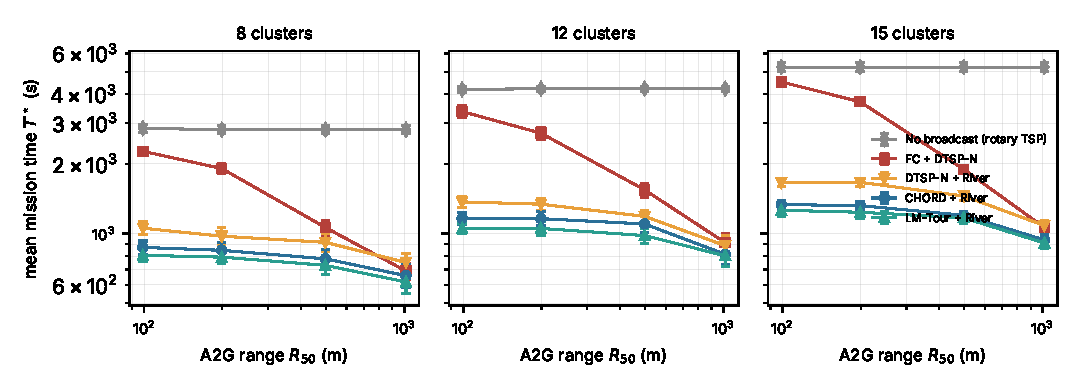
\includegraphics[width=0.86\textwidth]{tstar-c4.pdf}
\caption{Mean mission time versus A2G range, with 95\,\% confidence intervals over seeds.}\label{fig:tstar}
\end{figure*}

\textbf{Value of River.} DTSP-N+River against FC+DTSP-N isolates the ground transport: it is 14--23\,\% faster at 498\,m
and 49--63\,\% at 199 and 99\,m. Over open land it is not faster ($-3$ to $+9$\,\%): its zigzag path is longer than the
baseline's and River has little to move. River is a mechanism for short range.

\textbf{Choosing the path for the ground.} \lmtour{} is 10--26\,\% faster than DTSP-N+River although both use River and
the same tour solver. Flying close to every critical cell does not pay: on the 15-cluster map at 199\,m, \lmtour{} brings
only 36 of 92 critical cells within $\xi$ of the path (\chord{} 42, DTSP-N+River all 92) and is the fastest.
Against \chord{}, \lmtour{} is 1--11\,\% faster with a path 14--28\,\% shorter; the difference is significant (the
95\,\% interval of the paired per-seed difference excludes zero) in 10 of 12 settings.

\subsection{Anatomy of phase~1}
Table~\ref{tab:phase1} separates the flight from the ground. The flight of the River schemes is nearly independent of
the range, because the delivery constraint fixes the in-cluster time: on the 15-cluster map at 199\,m a pass takes 43.3\,s
with \chord{} (2099\,m at 48\,m/s), 40.5\,s with \lmtour{} (1560\,m at 38.5\,m/s) and 62.4\,s with DTSP-N+River (2438\,m),
whose path through every disc exceeds one copy of the query. FC+DTSP-N has the shortest tour over open land (30.5\,km on
the 8-cluster map) and by far the longest at short range (113\,km), where it orbits. The mean time at which critical
cells are ready, from take-off, is 58--106\,s earlier with \lmtour{} than with \chord{}; the difference in $T^\star$ is
smaller because phase~2 dilutes it.

\begin{table}[t]\centering
\caption{Phase~1 on the maps with 8 / 12 / 15 clusters: Team-1 flight time and mean time, from take-off, at which
critical cells are complete (s).}\label{tab:phase1}
\setlength{\tabcolsep}{2.5pt}\footnotesize
\begin{tabular}{llcc}\toprule
 & $R_{50}$ & flight & mean completion\\\midrule
FC+DTSP-N & 1016 & 669 / 913 / 1134 & \\
 & 498 & 1320 / 2011 / 2563 & \\
 & 199 & 2687 / 4016 / 5567 & \\
 & 99 & 3305 / 5078 / 6808 & \\\midrule
DTSP-N+River & 1016 & 1066 / 1553 / 2007 & 504 / 713 / 934\\
 & 99 & 1170 / 1589 / 2105 & 630 / 860 / 1066\\\midrule
\chord{}+River & 1016 & 784 / 1292 / 1437 & 360 / 566 / 701\\
 & 498 & 784 / 1292 / 1437 & 401 / 607 / 745\\
 & 199 & 784 / 1292 / 1437 & 438 / 643 / 777\\
 & 99 & 784 / 1292 / 1437 & 453 / 660 / 796\\\midrule
\lmtour{}+River & 1016 & 698 / 1085 / 1394 & 302 / 473 / 612\\
 & 498 & 699 / 1085 / 1308 & 338 / 508 / 654\\
 & 199 & 697 / 1083 / 1293 & 374 / 544 / 692\\
 & 99 & 708 / 1082 / 1291 & 389 / 554 / 705\\\bottomrule
\end{tabular}
\end{table}

\subsection{Ground transport: planning versus discovery}\label{sec:ground}
On the \chord{} passes of the 8-cluster map at $R_{50}=99$\,m, with five network realisations, we replace River by two
alternatives. \emph{Deluge}: advertise--request dissemination with Trickle timers ($I_{\min}=1$\,s, $I_{\max}=64$\,s,
$k=1$) and 64-packet pages aligned to image and segment boundaries, either on the cells of River's plan or only on the
\spine, the critical cells and the cells between them; radios are always on and there is no low-power listening.
\emph{Planned direct pull}: every critical cell asks each \spine{} cell for what it lacks along the shortest cell path,
with the same repair as River (two realisations).

\begin{table}[t]\centering
\caption{Ground transport on the same passes (8 clusters, $R_{50}=99$\,m), per cluster. Deluge: $\Delta$ is River minus
Deluge, mean $\pm$ 95\,\% CI over 40 (seed, cluster) pairs.}\label{tab:ground}
\setlength{\tabcolsep}{2pt}\scriptsize
\begin{tabular}{lccc}\toprule
 & River & Deluge, plan cells & Deluge, path cells\\\midrule
critical cells complete & 225/225 & 225/225 & 225/225\\
last critical cell ready (s) & 117 & 156 ($-39\pm12$) & 149 ($-32\pm12$)\\
frames sent ($10^3$) & 957 & 2344 ($-1386\pm139$) & 1786 ($-829\pm147$)\\
hop transmissions ($10^3$) & 432 & 1069 & 815\\
\quad of which control & 1.5 & 54.5 & 41.2\\
radio energy, always on (J) & 11\,059 & 14\,943 & 11\,001\\
radio energy, sched.\ sleep (J) & 1693 & 14\,943 & 11\,001\\
hottest node, sched.\ sleep (J) & 19.0 & 28.7 & 27.0\\
$T^\star$ (s) & 863 & 906 ($-43\pm8$) & 899 ($-36\pm7$)\\\bottomrule
\end{tabular}
\end{table}

Table~\ref{tab:ground} shows that all three deliver everything; River readies the last critical cell of a cluster
32--39\,s earlier, sends 1.9--2.5 times fewer frames, and lowers $T^\star$ by 36--43\,s. Two points qualify these numbers.

\emph{The saving is not control overhead.} Control frames are about 5\,\% of Deluge's transmissions. Deluge moves
1.7--2.2 times more \emph{data}, because every cell in scope must complete every page before it can advertise it, and it
is slower because each hop waits for a Trickle timer and a complete page. The energy advantage (6.5--8.8 times, CC2420
model \todo{datasheet citation}) comes from River's nodes sleeping after their last scheduled transmission while Deluge
must keep listening; with all radios always on the energies are within a factor 1.0--1.35. The sleeping figure is an
ex-post bound, optimistic in that it ignores wake-ups for repair requests.

\emph{The saving comes from planning.} Planned direct pull, which also knows in advance who holds what, matches River at
this range: 121 against 119\,s for the last critical cell and 873 against 870\,s for $T^\star$ on the two realisations
where both ran, with 11\,\% fewer frames. River's structure (Banks and Rings) pays off when paths to several critical
cells contend: on a single 80-cell cluster with four critical cells over open land it completes the last one 26\,\%
earlier with 12\,\% fewer frames than direct pulling, and with 4, 7 and 16 critical cells on a 91-cell cluster it uses
20--22\,\% fewer frames in 20 of 20 paired passes. What beats discovery is therefore the plan itself; the particular
shape of the plan matters in dense clusters.

\subsection{Trajectory error and takeover}\label{sec:wind}
The BS plans River on the intended path; the ns-3 pass flies a perturbed one. Lateral and along-track deviations are
white noise smoothed by a Gaussian kernel of 10\,s, with stationary standard deviation $\sigma$ laterally and $\sigma/2$
along the track; packet $s$ is still emitted at $s\Tp$, only its position changes. Flight tests of small fixed-wing
aircraft report cross-track errors of a few metres \cite{park2007,nelson2007}, so $\sigma=50$\,m is already
conservative; $\sigma=100$\,m is of the order of the overshoot of a turn planned in still air under strong wind
\cite{techy2009}, and equals the reception range of this regime. We use the 8-cluster map at $R_{50}=99$\,m, the
narrowest range, with three realisations.

\begin{table}[t]\centering
\caption{River under trajectory error (8 clusters, $R_{50}=99$\,m), without and with takeover: critical cells complete,
and readiness (per cluster, time of the last critical cell after the UAV leaves, mean over clusters; 900\,s if
incomplete).}\label{tab:wind}
\setlength{\tabcolsep}{2.5pt}\scriptsize
\begin{tabular}{cccc}\toprule
$\sigma$ (m) & seed & complete, without $\to$ with & readiness (s): on-plan / without / with\\\midrule
50 & 1 & 45 $\to$ 45 & 126 / 115 / 113\\
50 & 2 & 45 $\to$ 45 & 112 / 113 / 113\\
50 & 3 & 45 $\to$ 45 & 115 / 115 / 114\\
100 & 1 & 33 $\to$ 45 & 126 / 305 / 117\\
100 & 2 & 40 $\to$ 45 & 112 / 214 / 112\\
100 & 3 & 33 $\to$ 45 & 115 / 313 / 118\\\bottomrule
\end{tabular}
\end{table}

At $\sigma=50$\,m nothing breaks and takeover sends no frame (Table~\ref{tab:wind}). At $\sigma=100$\,m, River without
takeover completes only 106 of 135 critical cells and $T^\star$ rises by 294\,s; with takeover all 135 complete, readiness
returns to 112--118\,s (nominal 112--126\,s), and the mean $T^\star$ equals the on-plan value within run-to-run noise
($+0.2\pm121$\,s; per seed $-20$, $-35$, $+56$\,s, the same spread as at 50\,m where takeover is idle). In these runs the
holders are found from the real reception bitmaps without simulating the query. In a second implementation the \spine{}
cell floods a query over three cell hops with real control frames after the repair from adjacent cells has finished;
the results are unchanged: 135 of 135 complete, readiness 112--118\,s, total frames within $\pm3$\,\%, $T^\star$ minus
nominal $-22\pm184$\,s. (In a single realisation at $\sigma=200$\,m, which exceeds 1\,g of lateral acceleration at
times, River alone completes 3 of 45 critical cells and River with takeover 45 of 45.) The adaptive radius of
Algorithm~\ref{alg:takeover} is evaluated offline in Table~\ref{tab:radius}.

\subsection{Where to place the AI nodes}\label{sec:aicells}
So far $K$ was fixed by score outliers. Here $K$ is chosen, with the legacy cameras of Section~\ref{sec:model} sending,
before any incident, one record per passer-by to the nearest AI node of their cluster: a frame (40\,kB), a person crop
(10\,kB) or a feature vector (512-d INT8 plus 16\,B, 528\,B). Records travel only inside the mesh, from a camera to its
AI node; the BS still receives scores only. The background load uses the per-cell model fitted on the River trace (1.5 frames per
packet at the end cells, 1.7 in transit, 1 per gateway pair, 6.5\,ms per frame); every medium may be busy at most 10\,\% of
the time and 30\,\% of the nodes are cameras, each seen by $\rho$ people per hour.

\textbf{Which record.} On the 8-cluster map, with 8 to 128 AI cells placed by $k$-medoids, the largest $\rho$ under the
budget is 0.2--1.9 for frames, 0.7--7.7 for crops and 13--145 for vectors; the busiest medium is the cell of the AI node
itself. Frames and crops are therefore infeasible at any urban flow, and only vectors are kept. The 45 critical cells of
the outlier rule carry at most 18 people/h and lie up to 8 cells from some assigned node.

\textbf{Choosing $K$.} For each $\rho$ we take the fewest AI cells per cluster that keep the busiest medium under the
budget with every node at most $H=5$ cell hops from its AI cell (a capacitated facility location), placed by local search
on the River surrogate. Table~\ref{tab:aicells} lists the result: fewer than the outlier rule up to $\rho=50$, more above.
Fig.~\ref{fig:k9surr} checks the surrogate in ns-3 (both $R_{50}=199$ and 99\,m, one seed): up to 70 AI cells the
measured end of phase~1 is within 41\,s of the model and the order of the sets is kept, except that at 199\,m 69 AI
cells finish 12\,s after the outlier set instead of 41\,s before. With 161 AI cells (20 per cluster, outside the range
the surrogate was fitted on) the model fails: in one cluster ns-3 spreads from 75 to more than 900\,s, and phase~1 ends
at 1\,231\,s or later against 906\,s predicted.

\begin{table}[t]\centering\caption{AI cells needed and modelled end of phase~1 (s) at a 10\,\% budget, $R_{50}=99$\,m;
in brackets the ns-3 value (8 clusters, one seed).}\label{tab:aicells}
\begin{tabular}{lccc}\toprule
$\rho$ (people/h) & 8 clusters & 12 clusters & 15 clusters\\\midrule
20 & 24: 661 (687) & 32: 992 & 49: 1162\\
50 & 34: 674 & 52: 1005 & 64: 1168\\
100 & 69: 728 (733) & 98: 1061 & 123: 1235\\
200 & 161: 906 ($\ge$1231) & 220: 1147 & 275: 1362\\
outlier rule & 45: 753 (770) & 66: 1021 & 92: 1232\\\bottomrule
\end{tabular}\end{table}

\begin{figure}[t]\centering
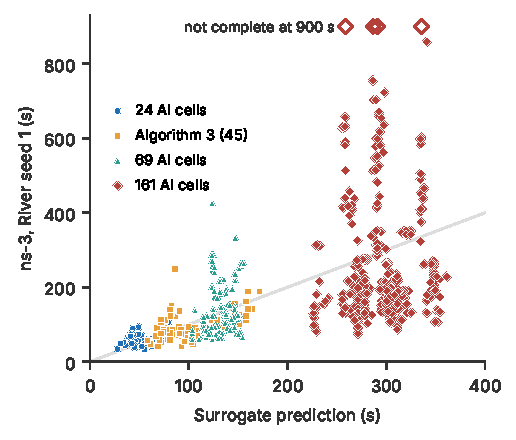
\includegraphics[width=0.9\columnwidth]{k9-surrogate-vs-ns3.pdf}
\caption{End of the query at each AI cell, from the UAV leaving its cluster: River surrogate versus ns-3, for the sets
chosen at $\rho=20$, 100 and 200 and for the outlier rule ($R_{50}=199$ and 99\,m, one seed). Hollow: not complete when
River stops at 900\,s.}\label{fig:k9surr}
\end{figure}

\textbf{Both phases.} Phase~2 follows the model of Section~\ref{sec:model} with verification by re-matching at the AI
node (5\,s to settle and 73\,s to send the full reference). An AI cell indexes $\rho\cdot 2\,\mathrm{h}\cdot 0.3\, n_c$
vectors for its $n_c$ assigned nodes and sets its threshold for a given false-alarm probability; the target passes a
uniformly drawn node. Fig.~\ref{fig:k9time} shows the time until the true AI cell is confirmed at $\rho=20$ (300 paired
draws). With a false-alarm probability of 0.1 per AI cell, the time grows from 823 to 1\,234\,s between 24 and 161 AI
cells, because the AI cells answering YES grow from 2.8 to 16.5. Holding the false alarms of the whole system at 2.4
narrows the gap (823 to 1\,061\,s) without reversing it, and the smaller set then also detects more often (0.63 against
0.58 with one target vector), since its per-cell threshold is lower. A larger index costs little detection: the
threshold grows with the logarithm of the index size.

\begin{figure}[t]\centering
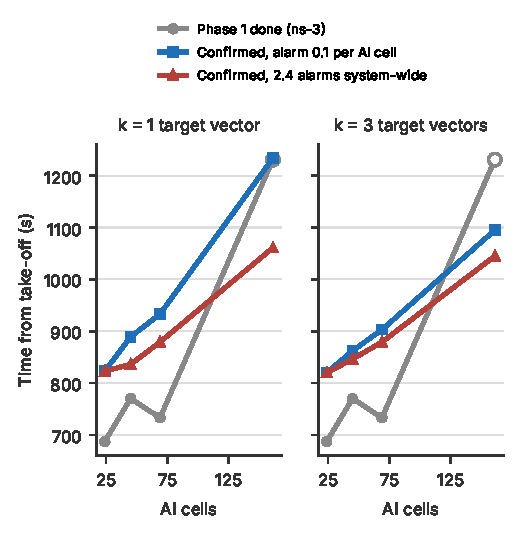
\includegraphics[width=\columnwidth]{k9-time-vs-ai-cells.pdf}
\caption{Time from take-off to the confirmation of the true AI cell versus the number of AI cells, $\rho=20$,
$R_{50}=99$\,m, under the two false-alarm rules; grey: last AI cell holding the query (hollow: lower bound).}\label{fig:k9time}
\end{figure}

\textbf{Sensitivity.} With an AI node in every cell, vectors fit up to $\rho=640$ people/h (1\,275 at a 20\,\% budget),
below a busy commercial street (about 1\,500) and a Manhattan peak (3\,700). All loads and index sizes scale with
$\rho$ times the camera share times the node density, so at 400 and 280 nodes/km$^2$ a set serves about 2.0 and 2.9
times the flow; thinning the nodes cell by cell confirms the scaling within 2\,\% for 24 AI cells but shows up to 23\,\%
more load for 161 AI cells at 280 nodes/km$^2$. The device tier does not change the choice: embedding one crop per
passer-by keeps an ESP32-class camera at most 28\,\% busy, and searching 152\,280 vectors with a 20-image reference takes
at most 5.4\,s at the AI node; only a microcontroller AI node needs external storage for the larger indexes (80\,MB).
\todo{second seed of the ns-3 check; River times at 400 and 280 nodes/km$^2$.}

\subsection{Stability across network realisations}
Differences between schemes that share River are stable across seeds (e.g., \lmtour{} minus DTSP-N+River on the
15-cluster map at 199\,m: $-425$\,s on the first seed, $-429\pm70$\,s on the others). Absolute values are not: with River,
$T^\star$ of other seeds is 56--197\,s above that of the first seed on the 15-cluster map, while a scheme that does not
depend on the mesh varies by $\pm15$\,s. The variation comes from the ns-3 network realisation (fading, MAC), which is
what a multi-seed campaign must capture; no number in this section relies on a single seed unless stated.
